\chapter{Binary Cahn--Hilliard: two free energies}
\label{ch:p1}

\begin{keybox}
\textbf{Key idea.} A blend of two components lowers its free energy by
\emph{demixing}. The Cahn--Hilliard equation is the conserved gradient
flow of a Ginzburg--Landau free energy; that free energy can only
decrease in time, and it splits into a \emph{bulk} (mixing) part and an
\emph{interfacial} (gradient) part whose competition sets the
morphology. Two quantitative predictions fall out of the same free
energy and we \emph{measure} both: the interface width and the
fastest-growing wavelength that the spinodal instability selects.
\end{keybox}

\begin{keybox}
\textbf{Learning objectives.} By the end you can: derive the conserved
Cahn--Hilliard flow from $F$ and split it into bulk and interfacial
parts; explain why $\ell\sim\sqrt{\kappa/W}$ (not $\sqrt\kappa$) and count
the cells it spans; predict $\lambda^\star=2\pi/k^\star$ and \emph{verify}
it against $S(q)$; keep apart the three ``energy decreases'' statements
and measure the last two; and report the cost of the Flory--Huggins
projection.\\[2pt]
\textbf{Prerequisites.} Calculus of variations ($\delta F/\delta c$),
Fourier modes, thermodynamics of mixing; Chapter~00 (environment green).
\emph{First physics chapter.}\\[2pt]
\textbf{Expected cost.} Any CUDA GPU, 2-D, $<1$\,GB device memory (an
8\,GB card is ample); solver \code{splu} (the CH saddle is indefinite).
Quick mode $\approx75$\,s wall (measured, RTX~6000 Ada; mostly kernel
compile); reference a few minutes; research (5-seed ensemble) tens of
minutes.
\end{keybox}

\section{The model}

Let $c(\mathbf{x},t)$ be the local volume fraction of one component (a
\emph{conserved} order parameter: the total amount of each species is
fixed). The Ginzburg--Landau free energy is
%
\begin{equation}
  F[c] \;=\; \intv \Big[\, f(c) \;+\; \tfrac{\kappa}{2}\,|\grad c|^2 \,\Big]\,dV ,
  \label{eq:F}
\end{equation}
%
with two contributions:
\begin{itemize}[nosep]
  \item the \textbf{bulk} (homogeneous) free energy density $f(c)$,
        which is minimized by the pure phases and \emph{penalized} in
        between --- this is what drives demixing. Write its scale as
        $W$, the height of the barrier between the two wells (units of
        energy/volume);
  \item the \textbf{interfacial} term $\tfrac{\kappa}{2}|\grad c|^2$,
        which penalizes spatial variation of $c$ and therefore
        \emph{opposes} demixing at short scales.
\end{itemize}

\begin{keybox}
\textbf{The interface width is $\ell\sim\sqrt{\kappa/W}$, not
$\sqrt{\kappa}$.} Balancing the gradient penalty against the bulk
barrier in \eqref{eq:F}, the equilibrium interface between the two
phases is a $\tanh$ profile of width
%
\begin{equation}
  \ell \;\sim\; \sqrt{\dfrac{\kappa}{W}} .
  \label{eq:width}
\end{equation}
%
Only the \emph{ratio} $\kappa/W$ is a length$^2$: $\kappa$ alone has
units of energy$\times$length$^2$/volume and cannot by itself set a
width. A deeper quench (larger $W$) sharpens the interface; a larger
$\kappa$ broadens it. For the symmetric polynomial well below
($W=1$ here) the exact profile gives $\ell=\sqrt{2\kappa/W}$, which at
the tutorial's $\kappa=5\times10^{-4}$ is $\POLYell$ (about
$\POLYellcells$ mesh cells --- comfortably resolved). We report the
width in physical length \emph{and} in cells so you can judge
resolution directly.
\end{keybox}

Because $c$ is conserved, the dynamics is the \emph{conserved}
(Model-B) gradient flow of \eqref{eq:F}: mass moves down gradients of
the chemical potential $\mu = \delta F/\delta c$,
%
\begin{equation}
  \dd{c}{t} = \grad\!\cdot\!\big(M\,\grad\mu\big),
  \qquad
  \mu = f'(c) - \kappa\,\grad^2 c .
  \label{eq:ch}
\end{equation}
%
Here $M>0$ is the mobility (it sets the \emph{time} scale but not the
equilibrium morphology). The fourth-order PDE is split into the two
second-order equations \eqref{eq:ch} --- the \emph{mixed} $(c,\mu)$ form
the solver uses.

\section{Two bulk free energies}

\paragraph{Polynomial double well (the canonical model).}
The simplest $f$ with two equal minima,
%
\begin{equation}
  f_{\text{poly}}(c) = \tfrac14\,(c^2-1)^2,\qquad
  f'=c^3-c,\qquad f''=3c^2-1,\qquad c\in[-1,1].
\end{equation}
%
The two phases are $c=\pm1$; the barrier height is $W=\tfrac14$ (and the
curvature scale that enters \eqref{eq:width} is order one, $|f''(0)|=1$).
The region $f''<0$ (i.e. $|c|<1/\sqrt3$) is \emph{spinodally unstable}.
This model is dimensionless and symmetric; it isolates the phase-field
mechanism from material detail.

\paragraph{Flory--Huggins (the physical model).}
For a real blend the mixing free energy is entropic $+$ enthalpic,
%
\begin{equation}
  f_{\text{fh}}(c) = A\,\big[c\ln c + (1-c)\ln(1-c)\big] + B\,c(1-c),
  \qquad c\in(0,1),
  \label{eq:fh}
\end{equation}
%
where the logarithmic \emph{entropy of mixing} (scale $A\sim 1/N$, with
$N$ the degree of polymerization) always favors mixing, and the
\emph{enthalpic} term $B\,c(1-c)$ (with $B$ the Flory interaction
parameter $\chi$) favors demixing. The curvature
%
\begin{equation}
  f_{\text{fh}}''(c) = A\Big(\tfrac1c + \tfrac1{1-c}\Big) - 2B
\end{equation}
%
is negative --- unstable --- only where the enthalpic $-2B$ beats the
entropic term. This is the \emph{spinodal}. The logs diverge at the
pure phases, so Flory--Huggins keeps $c$ strictly inside $(0,1)$, at the
cost of a stiff $f''$ near the walls.

\begin{keybox}
\textbf{Flory--Huggins needs a regularization \emph{and} a projection ---
and we report both.} Two numerical safeguards keep the logarithm usable,
and neither is free:
\begin{itemize}[nosep]
  \item \emph{Log regularization.} $\ln x$ is replaced by a $C^1$ linear
        extension below $x=\epsilon$ ($\epsilon=\FHregeps$), capping
        $f''$ at $1/\epsilon$ so a transient Newton overshoot near the
        wall does not produce an infinite Jacobian.
  \item \emph{Box projection.} Each Newton iterate is clipped back into
        $(0,1)$. This keeps the state physical, but clipping a conserved
        field \emph{moves mass}: when it fires it breaks exact
        conservation. We therefore report, for the run, the converged
        field bounds $\phi\in\FHcrange$ (strictly interior), the number
        of projected degrees of freedom, and the largest correction, so
        the cost of the safeguard is visible rather than hidden.
\end{itemize}
The distinction that matters: the projection fires on \emph{transient
Newton iterates} ($\FHprojdofs$ dof-clips over the reference run), but
each step's \emph{converged} state stays strictly interior
($\phi\in\FHcrange$), so no mass is moved on any accepted step and the
total mass is conserved to $\FHmass$. On a coarser mesh or a deeper
quench, though, Newton no longer resolves the interior state within its
iteration budget, the \emph{accepted} step is itself clipped, and mass
then drifts (the quick-mode $32^2$ run shows a
$\sim\!2\times10^{-4}$ drift for exactly this reason) --- a first,
concrete example of an admissibility safeguard trading conservation for
robustness (the substrate chapter, \ref{ch:p3}, returns to this with a
conservative correction).
\end{keybox}

\begin{keybox}
\textbf{Coefficients and their ranges.}
$M>0$ (mobility, time scale). $\kappa>0$ (gradient penalty; interface
width $\sqrt{\kappa/W}$ --- choose it so the interface spans a few mesh
cells). Polynomial: no free parameters, $W=\tfrac14$. Flory--Huggins:
$A>0$ (entropy, $\sim1/N$), $B=\chi$ (interaction; for $A=1$ the
symmetric point $c=\tfrac12$ is unstable once $B>2A=2$). The tutorial
uses $A=\FHA$, $B=\FHB$ (a clear quench); real blends map $A\sim1/N$,
$B\sim\chi$ (see \file{materials/materials.yaml}).
\end{keybox}

\section{Linear stability: the selected length scale}

Before any domains form, the nearly uniform blend is a superposition of
small Fourier modes. Linearizing \eqref{eq:ch} about the mean $\bar c$,
a mode $\propto e^{i\mathbf{k}\cdot\mathbf{x}+\sigma t}$ grows at rate
%
\begin{equation}
  \sigma(k) \;=\; -M\,k^2\big(f''(\bar c) + \kappa k^2\big).
  \label{eq:disp}
\end{equation}
%
When $f''(\bar c)<0$ a \emph{band} $0<k<k_c=\sqrt{-f''/\kappa}$ is
unstable, and one wavenumber grows fastest:
%
\begin{equation}
  k^\star = \sqrt{\dfrac{-f''(\bar c)}{2\kappa}},\qquad
  \lambda^\star = \dfrac{2\pi}{k^\star}.
  \label{eq:kstar}
\end{equation}
%
This $\lambda^\star$ is the wavelength the spinodal decomposition
\emph{selects} --- the initial domain spacing. For both free energies at
their (unstable) mean, $f''=\POLYfpp$, so
$k^\star=\POLYkstar$ and $\lambda^\star=\POLYlamstar$.

\begin{keybox}
\textbf{Prediction vs.\ measurement.} We verify \eqref{eq:disp}
directly. The quench is violent: with these coefficients the fastest
mode's growth rate is $\sigma^\star\!\sim\!M f''^2/(4\kappa)\!\sim\!500$,
so at the production time step the linear window is under one step. A
dedicated small-$\Delta t$ \emph{probe} (function \code{linear\_probe})
marches a few tiny steps from the small-amplitude initial field and
reads the growth of each Fourier shell,
$\sigma_{\text{meas}}(k)=\tfrac12\ln[S(k,\tau)/S(k,0)]/\tau$
(the factor $\tfrac12$ because $S\sim$ amplitude$^2$). Its peak lands on
the predicted $k^\star$: the measured fastest wavelength is $\POLYlammeas$
versus the predicted $\POLYlamstar$ (ratio $\POLYlamratio$), well within
one FFT shell. Figure~\ref{fig:p1disp} overlays the two.
\end{keybox}

\begin{figure}[h]\centering
  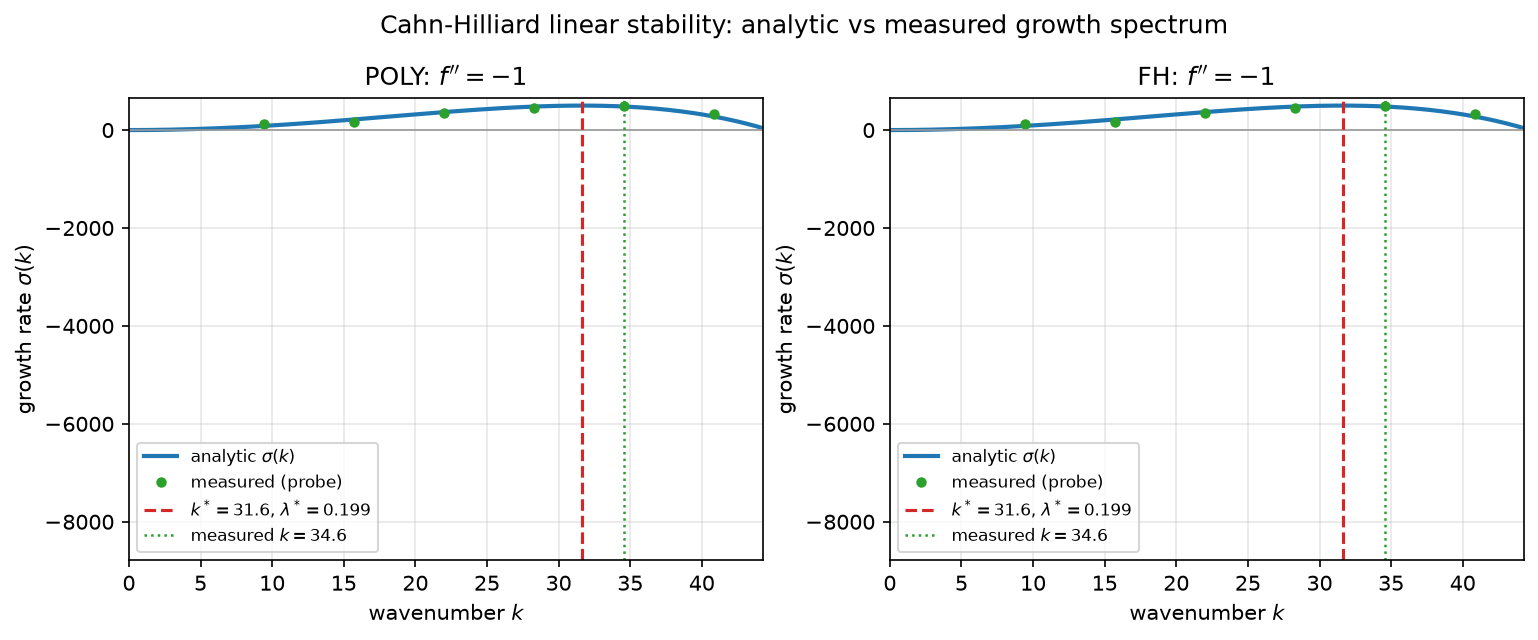
\includegraphics[width=\linewidth]{figures/p1_dispersion.png}
  \caption{Linear-stability dispersion. The analytic growth rate
    $\sigma(k)$ of \eqref{eq:disp} (line) against the measured growth
    spectrum from the small-$\Delta t$ probe (points), for the
    polynomial (left) and Flory--Huggins (right) free energies. The
    measured peak sits on the predicted fastest mode $k^\star$ (dashed),
    confirming that the spinodal selects $\lambda^\star=2\pi/k^\star$.}
  \label{fig:p1disp}
\end{figure}

\section{Run it}

\begin{runbox}
\textbf{Run it.}
\begin{lstlisting}
cd physics/01_ch_binary_energies
python run_harness.py --config configs/p1.yaml \
    --mode reference --output outputs/p1 --overwrite
python gen_figures.py --run-dir outputs/p1
\end{lstlisting}
The harness marches a spinodal decomposition for both free energies,
runs the linear-stability probe, tracks the energy budget and the
coarsening length scale, and checks the results against
\file{baseline.yaml} (tolerance-based invariants, not bit-identity).
\code{gen\_figures.py} renders every figure below from the saved
\file{results.json}/\file{history.npz} --- the document's numbers
\emph{are} the run's output. \file{quick} mode is a fast smoke; the
5-seed research ensemble is \file{--mode research}.
\end{runbox}

\paragraph{What you should see.}
From a nearly uniform, slightly noisy blend, fluctuations in the
unstable band grow at the rate \eqref{eq:disp}, the pattern sharpens
into domains of spacing $\sim\lambda^\star$ separated by interfaces of
width $\ell\sim\sqrt{\kappa/W}$, and then \emph{coarsens}. The total
free energy drops (after a one-step start-up transient), mass is
conserved to solver tolerance, and the field saturates at the two
coexisting phases.

\begin{keybox}
\textbf{Three statements about ``the energy decreases'' --- keep them
apart.}
\begin{enumerate}[nosep]
  \item \emph{Continuous Lyapunov.} In the PDE, $dF/dt =
        -\!\intv M|\grad\mu|^2\,dV\le0$ exactly. A theorem about the
        model.
  \item \emph{Discrete energy-stability.} Whether the \emph{time scheme}
        inherits $F^{n+1}\le F^{n}$ every step. This is a property of
        the discretization, not automatic. We measure it: the largest
        positive stepwise increment $\max_n(F^{n+1}-F^{n})$ after the
        start-up step is $\POLYlargestinc$ (polynomial) and
        $\FHlargestinc$ (Flory--Huggins) --- non-positive to round-off,
        so this scheme \emph{is} energy-stable here.
  \item \emph{One monotone run.} The particular trajectory you plotted
        went downhill. Necessary, not sufficient: report the increment,
        not just ``it looked monotone''.
\end{enumerate}
The step-$0\!\to\!1$ increment is separately reported ($\POLYstartup$
for the polynomial): the \code{mu\_init="consistent"} projection sets a
matching initial chemical potential so this start-up transient is small
and bounded, not an instability.
\end{keybox}

% --- generated by gen_figures.py ---
\begin{figure}[h]\centering
  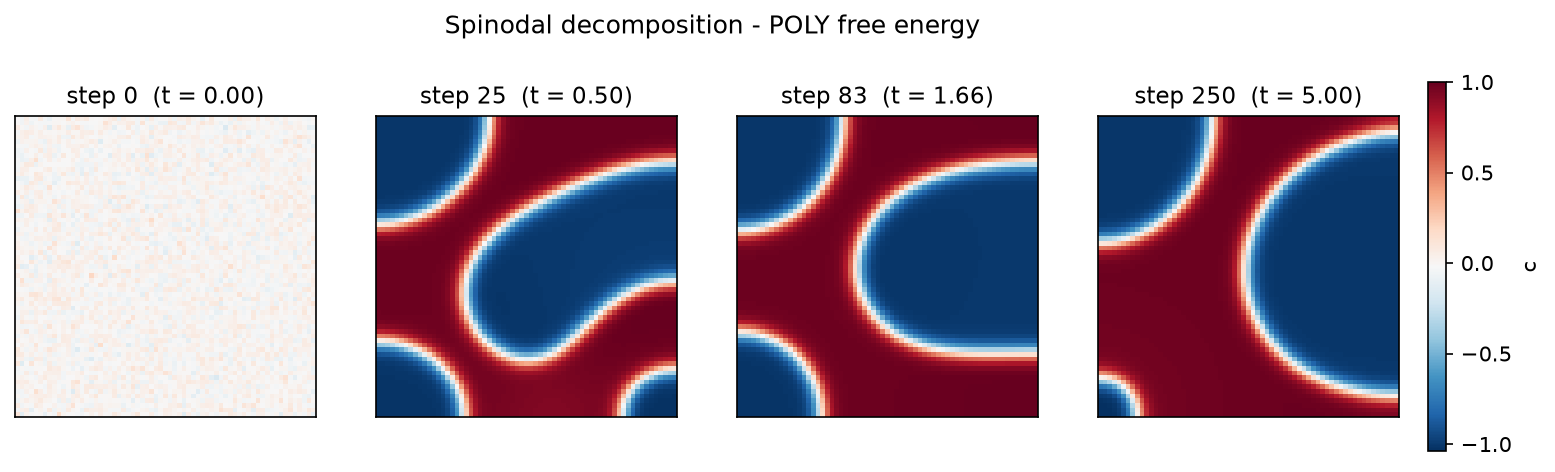
\includegraphics[width=\linewidth]{figures/p1_morph_poly.png}\\[4pt]
  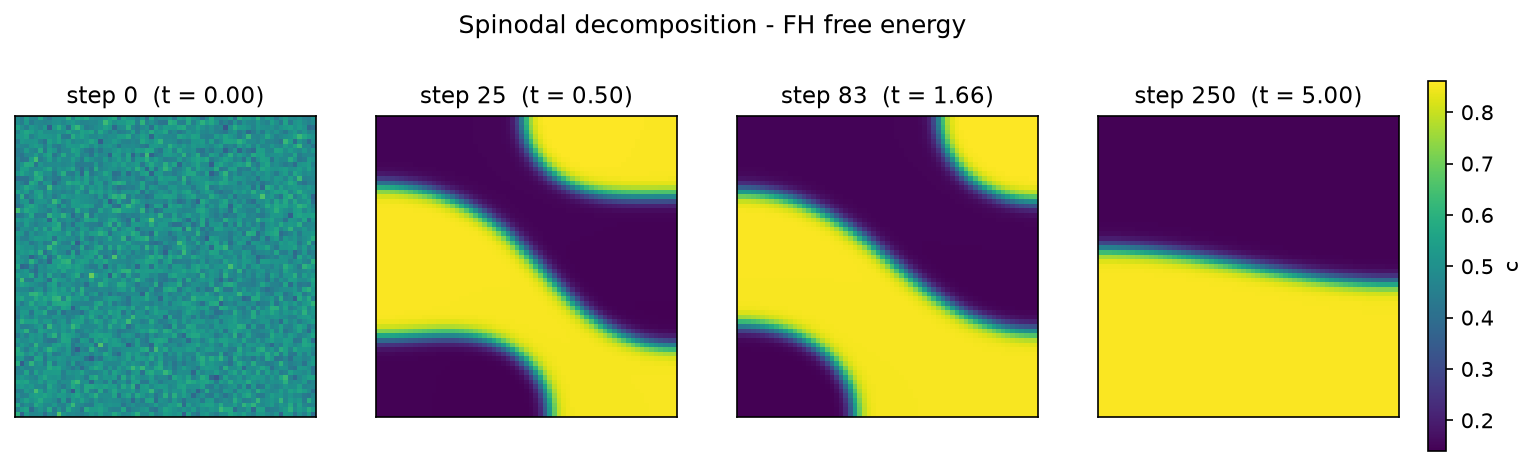
\includegraphics[width=\linewidth]{figures/p1_morph_fh.png}
  \caption{Spinodal decomposition and coarsening for the polynomial
    (top, $c\in[-1,1]$) and Flory--Huggins (bottom, $c\in(0,1)$) free
    energies. Same mixing physics, different order-parameter range and
    interface structure.}
  \label{fig:p1morph}
\end{figure}

\begin{figure}[h]\centering
  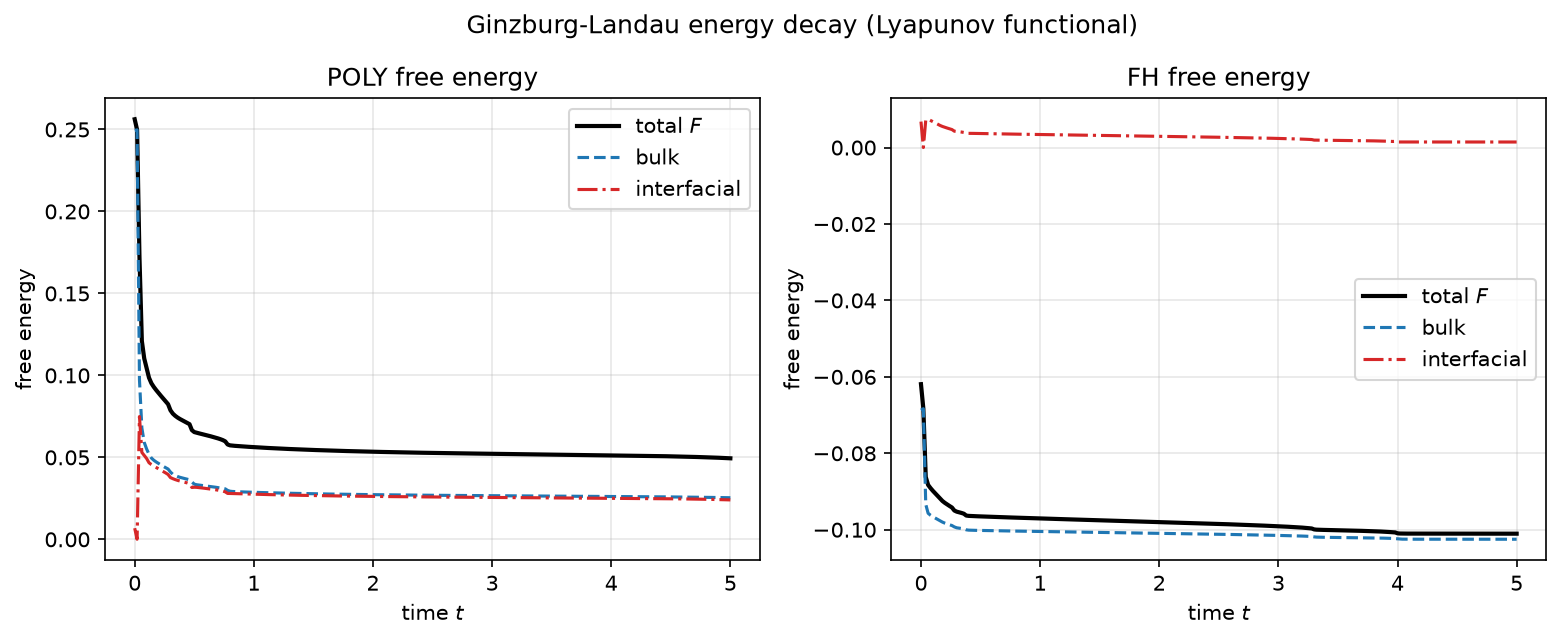
\includegraphics[width=\linewidth]{figures/p1_energy.png}
  \caption{The Ginzburg--Landau energy budget: total free energy (black)
    and its bulk (blue) and interfacial (red) parts versus time. Early
    on, forming interfaces \emph{raises} the interfacial energy while the
    bulk energy falls faster; during coarsening, domains merge and the
    interfacial energy falls as total interface area shrinks.}
  \label{fig:p1energy}
\end{figure}

\section{Coarsening: $L(t)\sim t^{n}$}

Once domains exist, they grow: interfacial energy is paid down by
merging domains, so the characteristic length $L(t)$ increases. We
measure $L(t)$ \emph{three} ways (all from the shared
\code{diffsim.diagnostics.morphology}) --- and the choice matters:
\begin{itemize}[nosep]
  \item \emph{peak} wavelength $2\pi/q_{\text{peak}}$ of the structure
        factor $S(q)$: the intuitive domain spacing, but on a coarse
        mesh it jumps between discrete $q$-shells (a quantization that
        shows up as a near-zero, poorly-fit exponent);
  \item \emph{first-moment} wavelength $2\pi/\langle q\rangle$:
        smoother, but biased low by the sharp-interface high-$k$ tail
        (it partly measures the interface width, not the domain size);
  \item \emph{interfacial-area} length $L=A_{\text{domain}}/P_{\text{int}}$
        (total area over total interface length): robust and monotone,
        because the interface shrinks as $\sim1/L$ during coarsening.
        This is the headline.
\end{itemize}
Fitting $L\sim t^{n}$ by least squares in $\log$--$\log$ on the
\emph{pre-saturation} window (skip the onset, cap at $L<\text{box}/3$
where finite-size saturation sets in --- the fit range is reported with
the number) gives, from the interfacial-area length,
$n=\POLYcoarsenN\pm\POLYcoarsenSD$ ($R^2=\POLYcoarsenR$) for the
polynomial well and $\FHcoarsenN\pm\FHcoarsenSD$ for Flory--Huggins ---
of order the diffusive Lifshitz--Slyozov value $n=\tfrac13$ for a
conserved order parameter, though the precise value is sensitive to the
length definition, the fit window, and finite-size saturation on the
small reference box (the research mode, on a larger box and longer
horizon, is where a clean asymptotic $1/3$ can be resolved). The peak
($n\!\approx\!\POLYcoarsenNpk$, quantization-limited) and first-moment
($n\!\approx\!\POLYcoarsenNfm$, tail-biased) definitions on the
\emph{same} run give very different slopes: a concrete lesson that a
coarsening exponent is only as good as the length definition, the fit
window, and the reported uncertainty --- never a single slope asserted
to be $1/3$.

\begin{figure}[h]\centering
  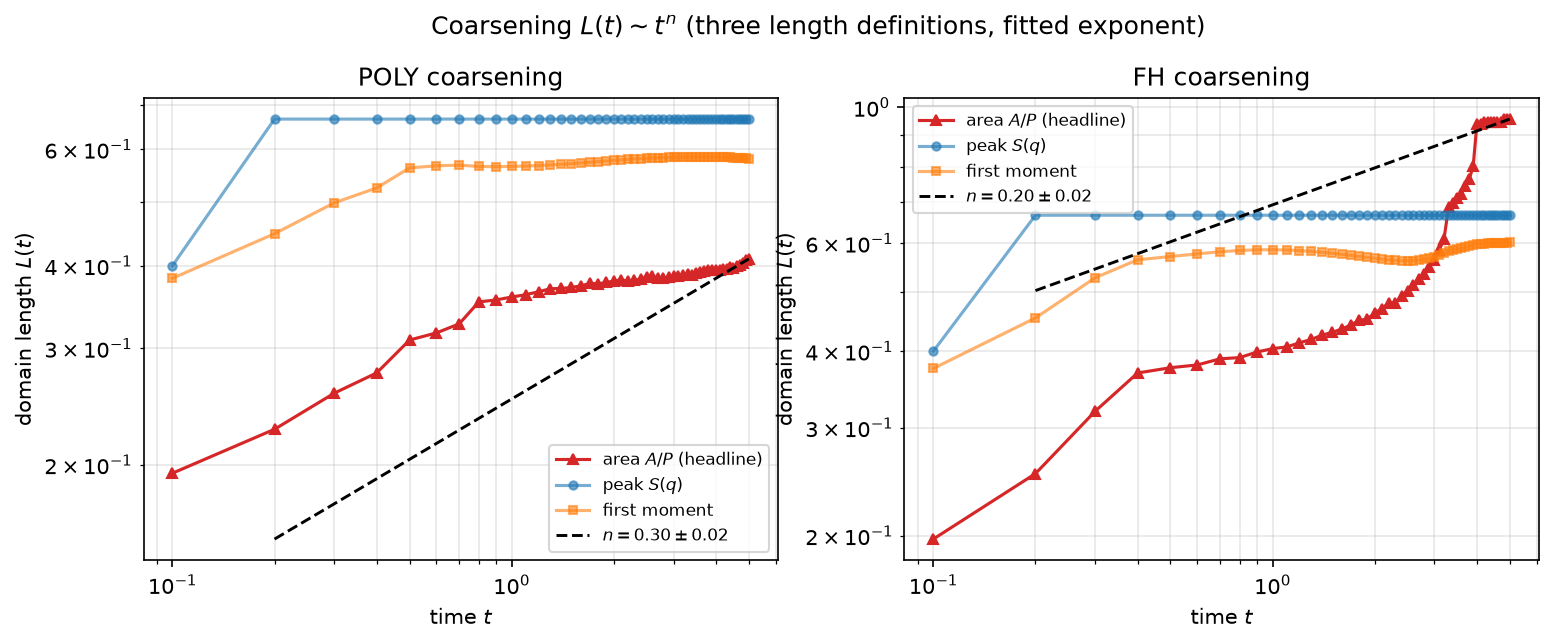
\includegraphics[width=\linewidth]{figures/p1_coarsening.png}
  \caption{Coarsening length $L(t)$ on log--log for the two free
    energies, from the peak (circles) and first-moment (squares)
    definitions of $S(q)$, with the fitted power law (dashed) and its
    uncertainty. The fit is taken on the coarsening window only.}
  \label{fig:p1coarsen}
\end{figure}

\begin{keybox}
\textbf{On the random seed --- and why the morphology is \emph{not}
reproducible.} The initial perturbation is drawn from a \emph{fixed}
seed so the figures here are reproducible \emph{on this machine}. But
the morphology is not a bit-reproducible quantity: which domain forms
where is chaotically sensitive to the seed, the mesh, and floating-point
order across GPUs. What \emph{is} robust is the physics --- the energy
decay, the selected wavelength $\lambda^\star$, the coarsening exponent,
the phase values $c_{\min},c_{\max}$. The research mode makes this
explicit: it runs a \textbf{5-seed ensemble} and reports the mean
$\pm$ standard deviation of the seed-independent quantities (final
energy, final length scale, exponent). The single fixed seed is for
the \emph{figures}; the science is the ensemble.
\end{keybox}

\begin{keybox}
\textbf{Measured self-check} (reference mode; your run reproduces these
within \file{baseline.yaml} tolerances, not bit-for-bit).
\begin{center}\small
\begin{tabular}{lcc}
\toprule
 & polynomial & Flory--Huggins \\
\midrule
total $F$: start $\to$ end       & \POLYFstart\ $\to$ \POLYFend & \FHFstart\ $\to$ \FHFend \\
interfacial energy: peak $\to$ end & \POLYFintpeak\ $\to$ \POLYFintend & \FHFintpeak\ $\to$ \FHFintend \\
interface width $\ell$ (cells)   & \POLYell\ (\POLYellcells) & \FHell\ (\FHellcells) \\
$\lambda^\star$: predicted / measured & \POLYlamstar\ / \POLYlammeas & \FHlamstar\ / \FHlammeas \\
coarsening $n$ (first moment)    & \POLYcoarsenN\ $\pm$ \POLYcoarsenSD & \FHcoarsenN\ $\pm$ \FHcoarsenSD \\
phase values $[c_{\min},c_{\max}]$ & \POLYcrange & \FHcrange \\
largest $+$ energy increment     & \POLYlargestinc & \FHlargestinc \\
mass drift $|\Delta m|$           & \POLYmass & \FHmass \\
projected dofs                    & \POLYprojdofs & \FHprojdofs \\
\bottomrule
\end{tabular}
\end{center}
\end{keybox}

\section{Code walk-through}

The tutorial's physics lives in \file{spinodal.py}, which drives the
production brick \file{src/diffsim/physics/cahn\_hilliard.py}; the
harness \file{run\_harness.py} turns it into a repeatable workflow, and
the measured quantities all come from the shared, unit-tested
\file{src/diffsim/diagnostics/} library (energy budget, structure
factor, admissibility, ensemble statistics).

\paragraph{1. Build a mesh and the stepper.}
\begin{lstlisting}
dm, mesh, cons = build_mesh_dm(level=6, p=1, device="cuda:0")  # 64x64
st = CahnHilliardStepper(dm, M, kappa, dt, order=1,
                         energy="poly")   # or energy="fh"
\end{lstlisting}
\code{energy} selects $f(c)$; \code{order} is the time scheme (1 =
backward Euler); \code{M}, \code{kappa} are the coefficients above.

\paragraph{2. Seed the initial blend.}
\begin{lstlisting}
st.set_initial(lambda x: c_avg + amp*rng.standard_normal(len(x)),
               mu_init="consistent")
\end{lstlisting}
A nearly uniform field with a small random perturbation --- the seed of
the spinodal instability. \code{mu\_init="consistent"} projects a
matching initial chemical potential so the first step sees no artificial
$\mu$-transient.

\paragraph{3. March, measure, verify.} \code{run\_spinodal} advances the
stepper, integrating the two energy densities of \eqref{eq:F} by the
same quadrature the solver uses and sampling the length scale $L(t)$ as
it goes; \code{linear\_probe} does the small-$\Delta t$ dispersion
verification; and the harness writes \file{results.json}, checks it
against \file{baseline.yaml}, and records provenance in
\file{metadata.json}.

\section{Explore on your own}

\question{Vary $\kappa$ over $\{2,5,10\}\times10^{-4}$. Confirm the
interface width scales as $\sqrt{\kappa/W}$ (not $\sqrt{\kappa}$) and
count the mesh cells it spans in each case. At what $\kappa$ does the
interface fall below $\sim$3 cells, and why should you stop trusting the
result there?}

\question{Verify the dispersion relation yourself: change $\bar c$ (for
Flory--Huggins) or $\kappa$ and check that the probe's measured fastest
mode tracks $k^\star=\sqrt{-f''/2\kappa}$. Where does $\bar c$ leave the
spinodal band ($f''>0$) and growth stop?}

\question{Run the 5-seed research ensemble. How large is the
seed-to-seed spread in the final energy and length scale compared with
the difference between the two free energies? Is the coarsening exponent
resolved within its uncertainty?}

\question{Extend the horizon (research mode, more steps). Does the
fitted coarsening exponent climb toward the Lifshitz--Slyozov $1/3$? Plot
$n$ versus fit-window start to see the asymptotic range emerge.}

\question{Drive Flory--Huggins into the wall: lower the mesh resolution
or deepen the quench ($B$ up) until the box projection fires. Watch
\code{proj\_dofs} and the mass drift rise together --- the safeguard
trading conservation for robustness.}

% ====================================================================
